\section{CIFAR10 Classification}
In this section we are going to demonstrate an end to end path to create a classifier for CIFAR10 dataset. 
\subsection{CIFAR}
The CIFAR-10 and CIFAR-100 are labelled subsets of the 80 million tiny images dataset. They were collected by Alex Krizhevsky, Vinod Nair, and Geoffrey Hinton \cite{cifar_report}. The CIFAR-10 dataset consists of 60000 32x32 colour images in 10 classes, with 6000 images per class. There are 50000 training images and 10000 test images.

We are working with CIFAR-10 dataset in this project. It comes as 3 pre created packages: Python, Matlab and Binary. As we are going to use python as  our programming language, we have utilized the python data package. It used the \textit{pickle} library to package the data.  Code samples are available on the original website to load the data as dictionaries in python. 

The data is available as 5 batches of training and one test batch.  Once loaded in python, each batch, gives you a $10000 \times 3072 $ matrix as input vectors. In the same time  is provides a label vector $10000 \times 1$ with numbers between 0, 9 defining the class of each data point.  In order to use the labels on our code simple conversion to 0-1 matrix is required. 

\subsection{Network}
As part of this homework we supposed to create the basis for training neural networks. In this part I want to talk more about the code that been written. 

We have a class called \textit{GraphNetwork} It is simply a network of layers (nodes) tied together to perform the calculations for forward and backward pass. Each network will have a number of input nodes. Each input is like a data batch supposed to be processed.  Then we add nodes of various types to the network to build what we want to do. Here is the list of various Layer(node) types available in our codebase: 
\begin{itemize}
    \item \textbf{HiddenLayer} A fully connected layer with different activation functions (currently only \textit{tanh} and \textit{Relu} are supported)
    \item \textbf{BiasLayer} This layer appends one constant dimension to the end of the input and augment the input with one extra dimension. 
    \item \textbf{ConcatenateLayer} This layer concatenate multiple inputs into single matrix 
    \item \textbf{SoftmaxLayer}  This layer calculates the softmax of it's inputs 
    \item \textbf{CrossEntropyLayer} This layer calculates the cross entropy of two input matrices.  
    \item \textbf{RMSLayer} This layer calculates the elementwise square distance of two matrices
    \item \textbf{BatchSumLayer} This layer calculates the sum of all entries of it's inputs. 
\end{itemize}

For all of the above layers we have written the forward and backward pass. In the forward pass the normal flow is calculated. In backward pass it accepts the loss gradient and also the original input values, then it calculates the gradients for the inputs and parameters of the layer.  In the above list of layers currently only the HiddenLayer supports the back prop as it has internal parameters. Others simply only calculate the backward flow of the network and no back prop is applied on them. 


The GraphNetwork is then responsible to run the layers in the proper order and also get the gradients and calculated the backward flow.  It simply uses the topological sort of the nodes to run them one by one.  
\subsubsection{Empirical Gradient}
To make sure that we hade properly calculated the gradients,  We applied the empirical gradient calculation. In this method a complex network which contains all of the above nodes is created. Then we simply change a parameter in hidden layer and calculate the difference in output value of the network. So it only involves calculation of the forward pass.

\begin{equation*}
    \frac{\partial L}{\partial w_{ij}} \approx  \frac{L^{\prime} - L}{\Delta}
\end{equation*}

Fortunately this method helped a lot to find the bugs in implementation. 
One of the funny things that happened during test was that the test network had a SumLayer after Softmax and the gradient was always zero. It took a while to find out that the sum of a SoftMax is always 1 and it is logical to have a zero gradient. 

\subsubsection{Toy Problem}
After gradients looked fine it was the time to check the behaviour of network with simple interpolation task. 
The task was to interpolate following function 
\begin{equation*}
    f(X) = \sum_{i = 0}^{ D} x_i ^ 2 + 5 x_i 
\end{equation*}

The $D = 20$ is the dimension of the input space. The network architecture was a two hidden layers and at the end a RMS element. 

We started with \textit{tanh} as activation function, but it drastically failed the challenge. It  could not capture the inputs at all. 

Here is the list of layers: 
\begin{enumerate}
    \item  InputLayer ($4000 \times 20 $ data points)
    \item BiasLayer 
    \item HiddenLayer 1: Various activation functions tested with 10 neurons     
    \item BiasLayer 
    \item HiddenLayer 2: Linear activation function used (means no activation basically). With one neuron only. 
    \item RMSLayer 
    \item BatchSumLayer 
\end{enumerate}

Here is  the performance of the network:

\begin{figure}[!htb]
    \centering
    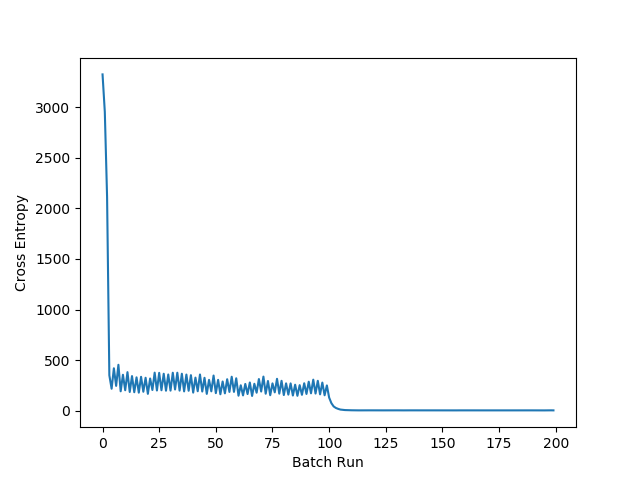
\includegraphics[scale=0.7]{images/quadratic_performance_linear.png}
    \caption{Performance on Quadratic Function Estimation Linear Activation function}
\end{figure}

\subsection{Data Pre-process}
As basic step we performed pre-process on the data. It starts with  reducing the data dimension by making them mono chrome. This reduces the input vector from 3072 to 1024.  

Also we are normalizing the input vectors by making them zero centred. As all of the inputs are from the same nature (pixel intensities) there is no need for whitening.

\subsection{Training }
We tried multiple architectures to explore the  task performance.  I will try to tell the story here as the results are not as satisfactory as expected.

Here is the base architecture: 
\begin{enumerate}
    \item InputLayer ($N \times 1024 $ data points)
    \item BiasLayer 
    \item HiddenLayer 1: Various activation functions tested with 10 neurons     
    \item BiasLayer 
    \item HiddenLayer 2: Linear activation function used (means no activation basically). With one neuron only. 
    \item SoftmaxLayer
    \item CrossEntropyLayer
    \item BatchSumLayer 
\end{enumerate}

Initially all configurations tested we were not able to go down the random cross entropy ($ln 10 \approx 2.3 $  is the performance of random classifier).  Here is the summary of try and error plus learning we had: 

\begin{itemize}
    \item The network starts with very high error rates. My expectation was to start from random point. Funny enough it takes good number of epochs to reach the average point of cross entropy of random classifier. 
    \item We started with small number of samples to check if network can overfit them or not. Unfortunately even with small number of samples network was not able to pass through the random point. 
    \item I was trying to reduce the  learning rate once we were stuck in the plateau, but it didn't work 
    \item Then by printing the gradients I realized that initially they are very large but as we go forward they become very small. My learning rates where in order of $10^{-6}$  it become obvious that I have to increase the learning rate. 
    \item So initially we start with small learning rate, once the network reaches the random error state, we increase the learning rate.  With this trick the loss function drops into values  around 0.9 which is one third of the initial random value. But unfortunately gets stuck there. 
    \item  I made a change and changed the second layer to be simply a linear, this was like a miracle. It allowed the network to be traind normally> I cannot beleive such a small change caused such a big improvement in the performance of the network.
\end{itemize}